\section{Praktika ekzerco}
\subsection{Uzantkontoj}
%%%>>>>>>>>>>>>>>>>>>>>>>>>>>>>>>>>>>>>>>>>>>>>>>>>>>>>>>>>>>>>>>>>>>>>>>>>>>>>>>>>>>>>>>>>>>>>>>
  \begin{frame}
    \frametitle{Ensalutu en trellon}

	Uzu sian propran Trello konton, Google konton aŭ uzu unu el la subaj:

\begin{center}
	\begin{tabular}{ | c | c | }
	\hline
		uzantnomo & pasvorto \\
	\hline
		blanka.anasero{@}gmail.com & 2anaseroj \\
	\hline
		griza.alaudo{@}gmail.com & 2alaudoj \\
		
%		najtingalo\_trejnanto{@}gmail.com & 2najtingaloj \\
%		kolombo\_trejnanto{@}gmail.com & 2kolomboj\\
	\hline  
	\end{tabular}
\end{center}

\end{frame}
%%%<<<<<<<<<<<<<<<<<<<<<<<<<<<<<<<<<<<<<<<<<<<<<<<<<<<<<<<<<<<<<<<<<<<<<<<<<<<<<<<<<<<<<<<<<<<<<<

%%%>>>>>>>>>>>>>>>>>>>>>>>>>>>>>>>>>>>>>>>>>>>>>>>>>>>>>>>>>>>>>>>>>>>>>>>>>>>>>>>>>>>>>>>>>>>>>>
  \begin{frame}
    \frametitle{Fulmklavoj}
    \framesubtitle{Provu ilin uzi ekzercante!}
    
    \begin{columns}
    \column{0.6\textwidth}
	
	Memoru nur, ke:    
    
	\begin{itemize}
		\item Per klavo ? vi povas rigardi fulmklavaron.
		\item Tre indas tion fari ofte kaj lerni paŝo post paŝo.
	\end{itemize}
    
    	
	\column{0.4\textwidth}
    
    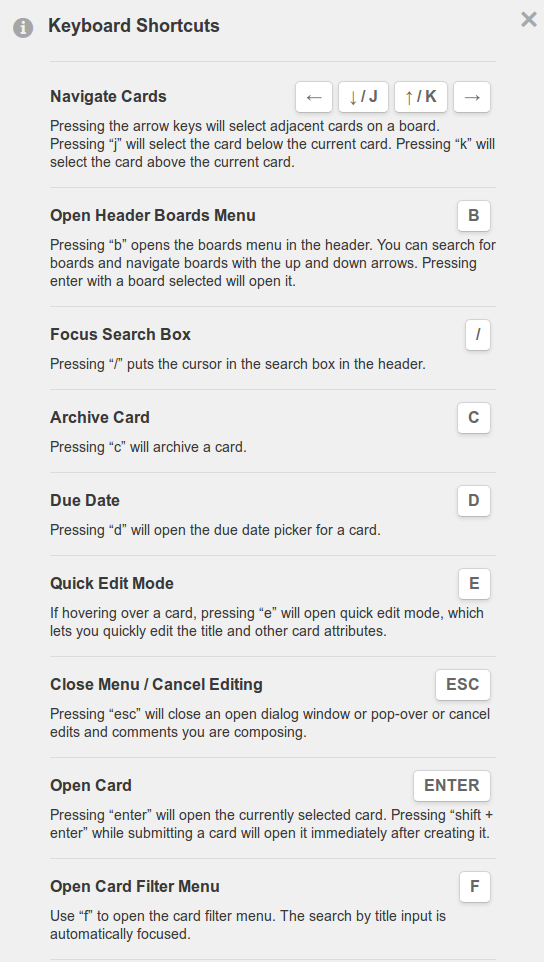
\includegraphics[scale=0.2]{ekranoj/fulmklavaro}
	
	\end{columns}
	
	
  \end{frame}
%%%<<<<<<<<<<<<<<<<<<<<<<<<<<<<<<<<<<<<<<<<<<<<<<<<<<<<<<<<<<<<<<<<<<<<<<<<<<<<<<<<<<<<<<<<<<<<<<




\subsection{Para klakado}
%%%>>>>>>>>>>>>>>>>>>>>>>>>>>>>>>>>>>>>>>>>>>>>>>>>>>>>>>>>>>>>>>>>>>>>>>>>>>>>>>>>>>>>>>>>>>>>>>
  \begin{frame}
    \frametitle{Pariĝu!}
    
    \begin{enumerate}

		\item Decidu kiu unue estos gufujdiĵoranto, kiu gufujkliento.
		\item Ambaŭ personoj havu iun ajn aliron al Trello: telefona aŭ (tabul)komputila. Prefere samtempe, se mankos iloj ni atendos ĝis ĉiuj paroj finos.
		\item Flanka peto: ne malpurigu la komputilojn! :-)
    
    \end{enumerate}
  \end{frame}
%%%<<<<<<<<<<<<<<<<<<<<<<<<<<<<<<<<<<<<<<<<<<<<<<<<<<<<<<<<<<<<<<<<<<<<<<<<<<<<<<<<<<<<<<<<<<<<<<


%%%>>>>>>>>>>>>>>>>>>>>>>>>>>>>>>>>>>>>>>>>>>>>>>>>>>>>>>>>>>>>>>>>>>>>>>>>>>>>>>>>>>>>>>>>>>>>>>
  \begin{frame}
    \frametitle{Ekzerco}
    \framesubtitle{Parto unua}

	\begin{itemize}
		\item Diĵoranto:
		\begin{enumerate}
			\item Kreu tabulon "Posttagmeza menuo".
			\item Agordu tiel, ke la nuraj listoj estu: MENDOJ, SERVITAJ, MENUO.
			\item Aldonu du kartojn: "Vaflo kun dolĉa ŝmiraĵo", "Teo".
			\item Aldonu la klienton al la tabulo.
		\end{enumerate}
			
		\item Kliento:
		\begin{enumerate}
			\item Mendu dolĉaĵon (kreu taŭgan karton en la taŭga listo).
			\item Aldonu la diĵoranton al la karto.
		\end{enumerate}    
	\end{itemize}
	    
  \end{frame}
%%%<<<<<<<<<<<<<<<<<<<<<<<<<<<<<<<<<<<<<<<<<<<<<<<<<<<<<<<<<<<<<<<<<<<<<<<<<<<<<<<<<<<<<<<<<<<<<<

%%%>>>>>>>>>>>>>>>>>>>>>>>>>>>>>>>>>>>>>>>>>>>>>>>>>>>>>>>>>>>>>>>>>>>>>>>>>>>>>>>>>>>>>>>>>>>>>>
  \begin{frame}
    \frametitle{Ekzerco}
    \framesubtitle{Parto dua}

	\begin{itemize}
			
		\item Diĵoranto:
		\begin{enumerate}
			\item Kreu markoliston kun jenaj paŝoj:
				\begin{enumerate}
					\item Difini kia ŝmiraĵo
					\item Servado
					\item Pagado
				\end{enumerate}
				
			\item Demandu kia ŝmiraĵo kaj metu klienton sur la karto.
		\end{enumerate}
				
    
		\item Kliento:
		\begin{enumerate}
			\item Respondu pri ŝmiraĵo, marku ĝustan paŝon sur la markolisto.
			\item Remetu diĵoranton al la karto.
		\end{enumerate}    
		
		\item Diĵoranto:
		\begin{enumerate}
			\item Servu, marku markoliston.
			\item Metu la karton en "SERVITAJ" listo.
		\end{enumerate}    
			
	\end{itemize}		
	
    
  \end{frame}
%%%<<<<<<<<<<<<<<<<<<<<<<<<<<<<<<<<<<<<<<<<<<<<<<<<<<<<<<<<<<<<<<<<<<<<<<<<<<<<<<<<<<<<<<<<<<<<<<


%%%>>>>>>>>>>>>>>>>>>>>>>>>>>>>>>>>>>>>>>>>>>>>>>>>>>>>>>>>>>>>>>>>>>>>>>>>>>>>>>>>>>>>>>>>>>>>>>
  \begin{frame}
    \frametitle{Esenco}
    
	Vi ĉiam strebu \alert{forigi sian vizaĝon de la karto} per:
    
    \begin{itemize}
    	\item plenumo de la peto/tasko,
    	\item klarigo kial ne vi taŭgas (ĉiam trovu anstataŭanton),
    	\item aliaj laŭ via kreemeco, kondiĉe ke kun \alert{fortaj argumentoj} por tio.
    \end{itemize}
    
  \end{frame}
%%%<<<<<<<<<<<<<<<<<<<<<<<<<<<<<<<<<<<<<<<<<<<<<<<<<<<<<<<<<<<<<<<<<<<<<<<<<<<<<<<<<<<<<<<<<<<<<<

